% 2006_shanghai_spring_q17_fig1: cuboid ABCD-A1B1C1D1 with diagonals A1B and B1C
% schematic oblique projection; topology from original PNG
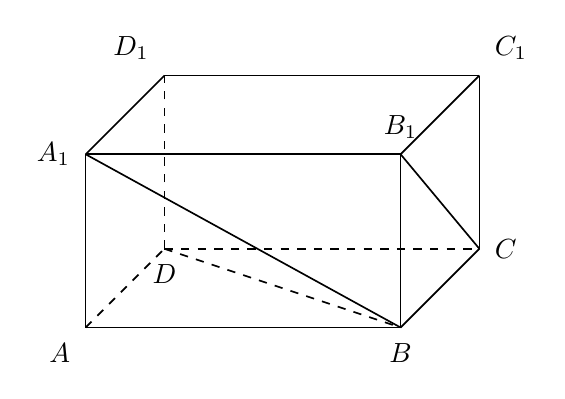
\begin{tikzpicture}[x=1cm,y=1cm,font=\normalsize,line width=.6pt]
\coordinate (A) at (0,0);
\coordinate (B) at (4,0);
\coordinate (C) at (5,1);
\coordinate (D) at (1,1);
\coordinate (A1) at (0,2.2);
\coordinate (B1) at (4,2.2);
\coordinate (C1) at (5,3.2);
\coordinate (D1) at (1,3.2);
% cuboid visible edges
\draw[solid] (A) -- (B);
\draw[solid] (B) -- (C);
\draw[solid] (C) -- (C1);
\draw[solid] (C1) -- (D1);
\draw[solid] (D1) -- (A1);
\draw[solid] (A1) -- (A);
\draw[solid] (A1) -- (B1);
\draw[solid] (B1) -- (B);
\draw[solid] (B1) -- (C1);
% cuboid hidden edges
\draw[dashed] (A) -- (D);
\draw[dashed] (D) -- (C);
\draw[dashed] (D) -- (D1);
% required diagonals from problem figure
\draw[solid] (A1) -- (B);
\draw[solid] (B1) -- (C);
% base diagonal visible as dashed in original
\draw[dashed] (D) -- (B);
% labels
\node[below left=2pt] at (A) {$A$};
\node[below=2pt] at (B) {$B$};
\node[right=2pt] at (C) {$C$};
\node[below=2pt] at (D) {$D$};
\node[left=2pt] at (A1) {$A_{1}$};
\node[above=2pt] at (B1) {$B_{1}$};
\node[above right=2pt] at (C1) {$C_{1}$};
\node[above left=2pt] at (D1) {$D_{1}$};
\end{tikzpicture}
